\begin{appendix}

\chapter{Appendix}
\label{chap:Appendix}

% This is the place for extensive derivations and secondary data which would otherwise hamper the readability of the proper thesis\\

% All details that were not used in the main part of the thesis are summed up in the appendix, such as mathematical derivations, source codes, long tables, lists of results etc.

% \begin{algorithm}[H]
%  \KwData{this text}
%  \KwResult{how to write algorithm with \LaTeX2e }
%  initialization\;
%  \While{not at end of this document}{
%   read current\;
%   \eIf{understand}{
%    go to next section\;
%    current section becomes this one\;
%    }{
%    go back to the beginning of current section\;
%   }
%  }
%  \caption{How to write algorithms}
% \label{ap:dev_alg}

% \end{algorithm}

\begin{figure}[!ht]
	\centering
    \def\svgwidth{.8\linewidth}
    \small\input{figures/mic_rec_setup.pdf_tex}
	% 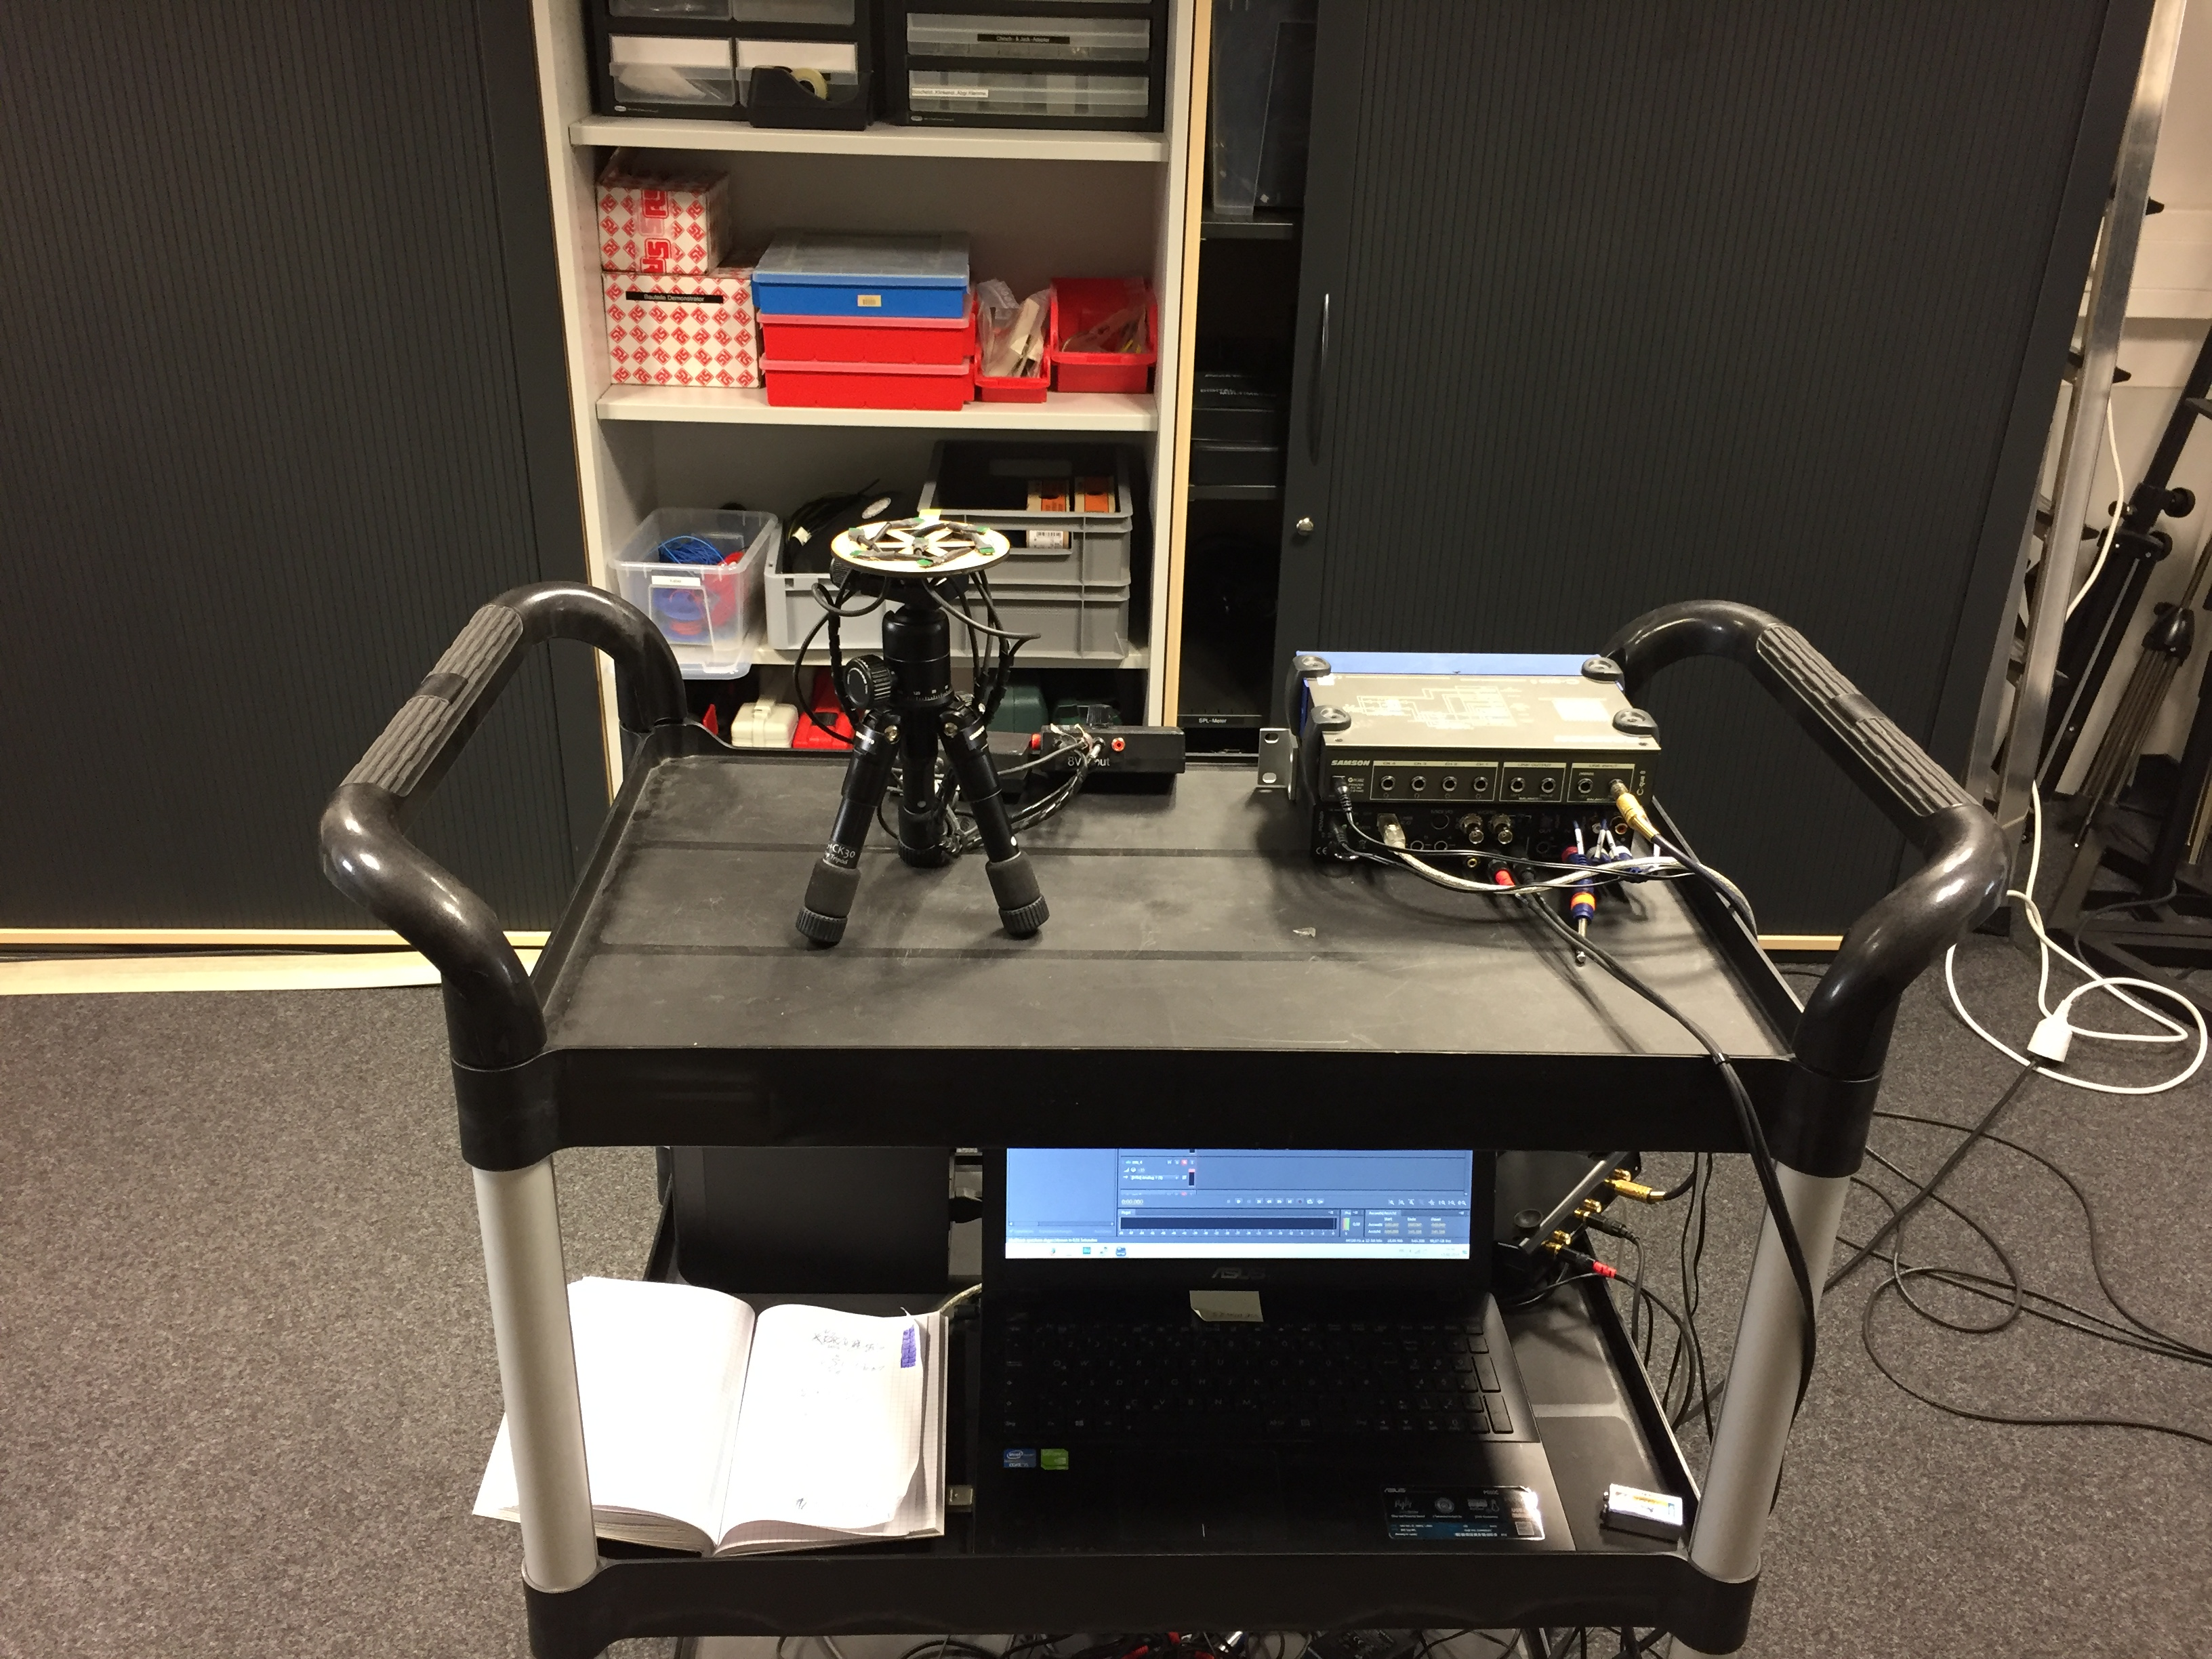
\includegraphics[width=0.8\textwidth]{figures/mic_rec_setup.jpg}
	\caption{Microphone signal recording setup}
	\label{fig:mic_rec_setup}
\end{figure}

\begin{figure}[!ht]
	\centering
	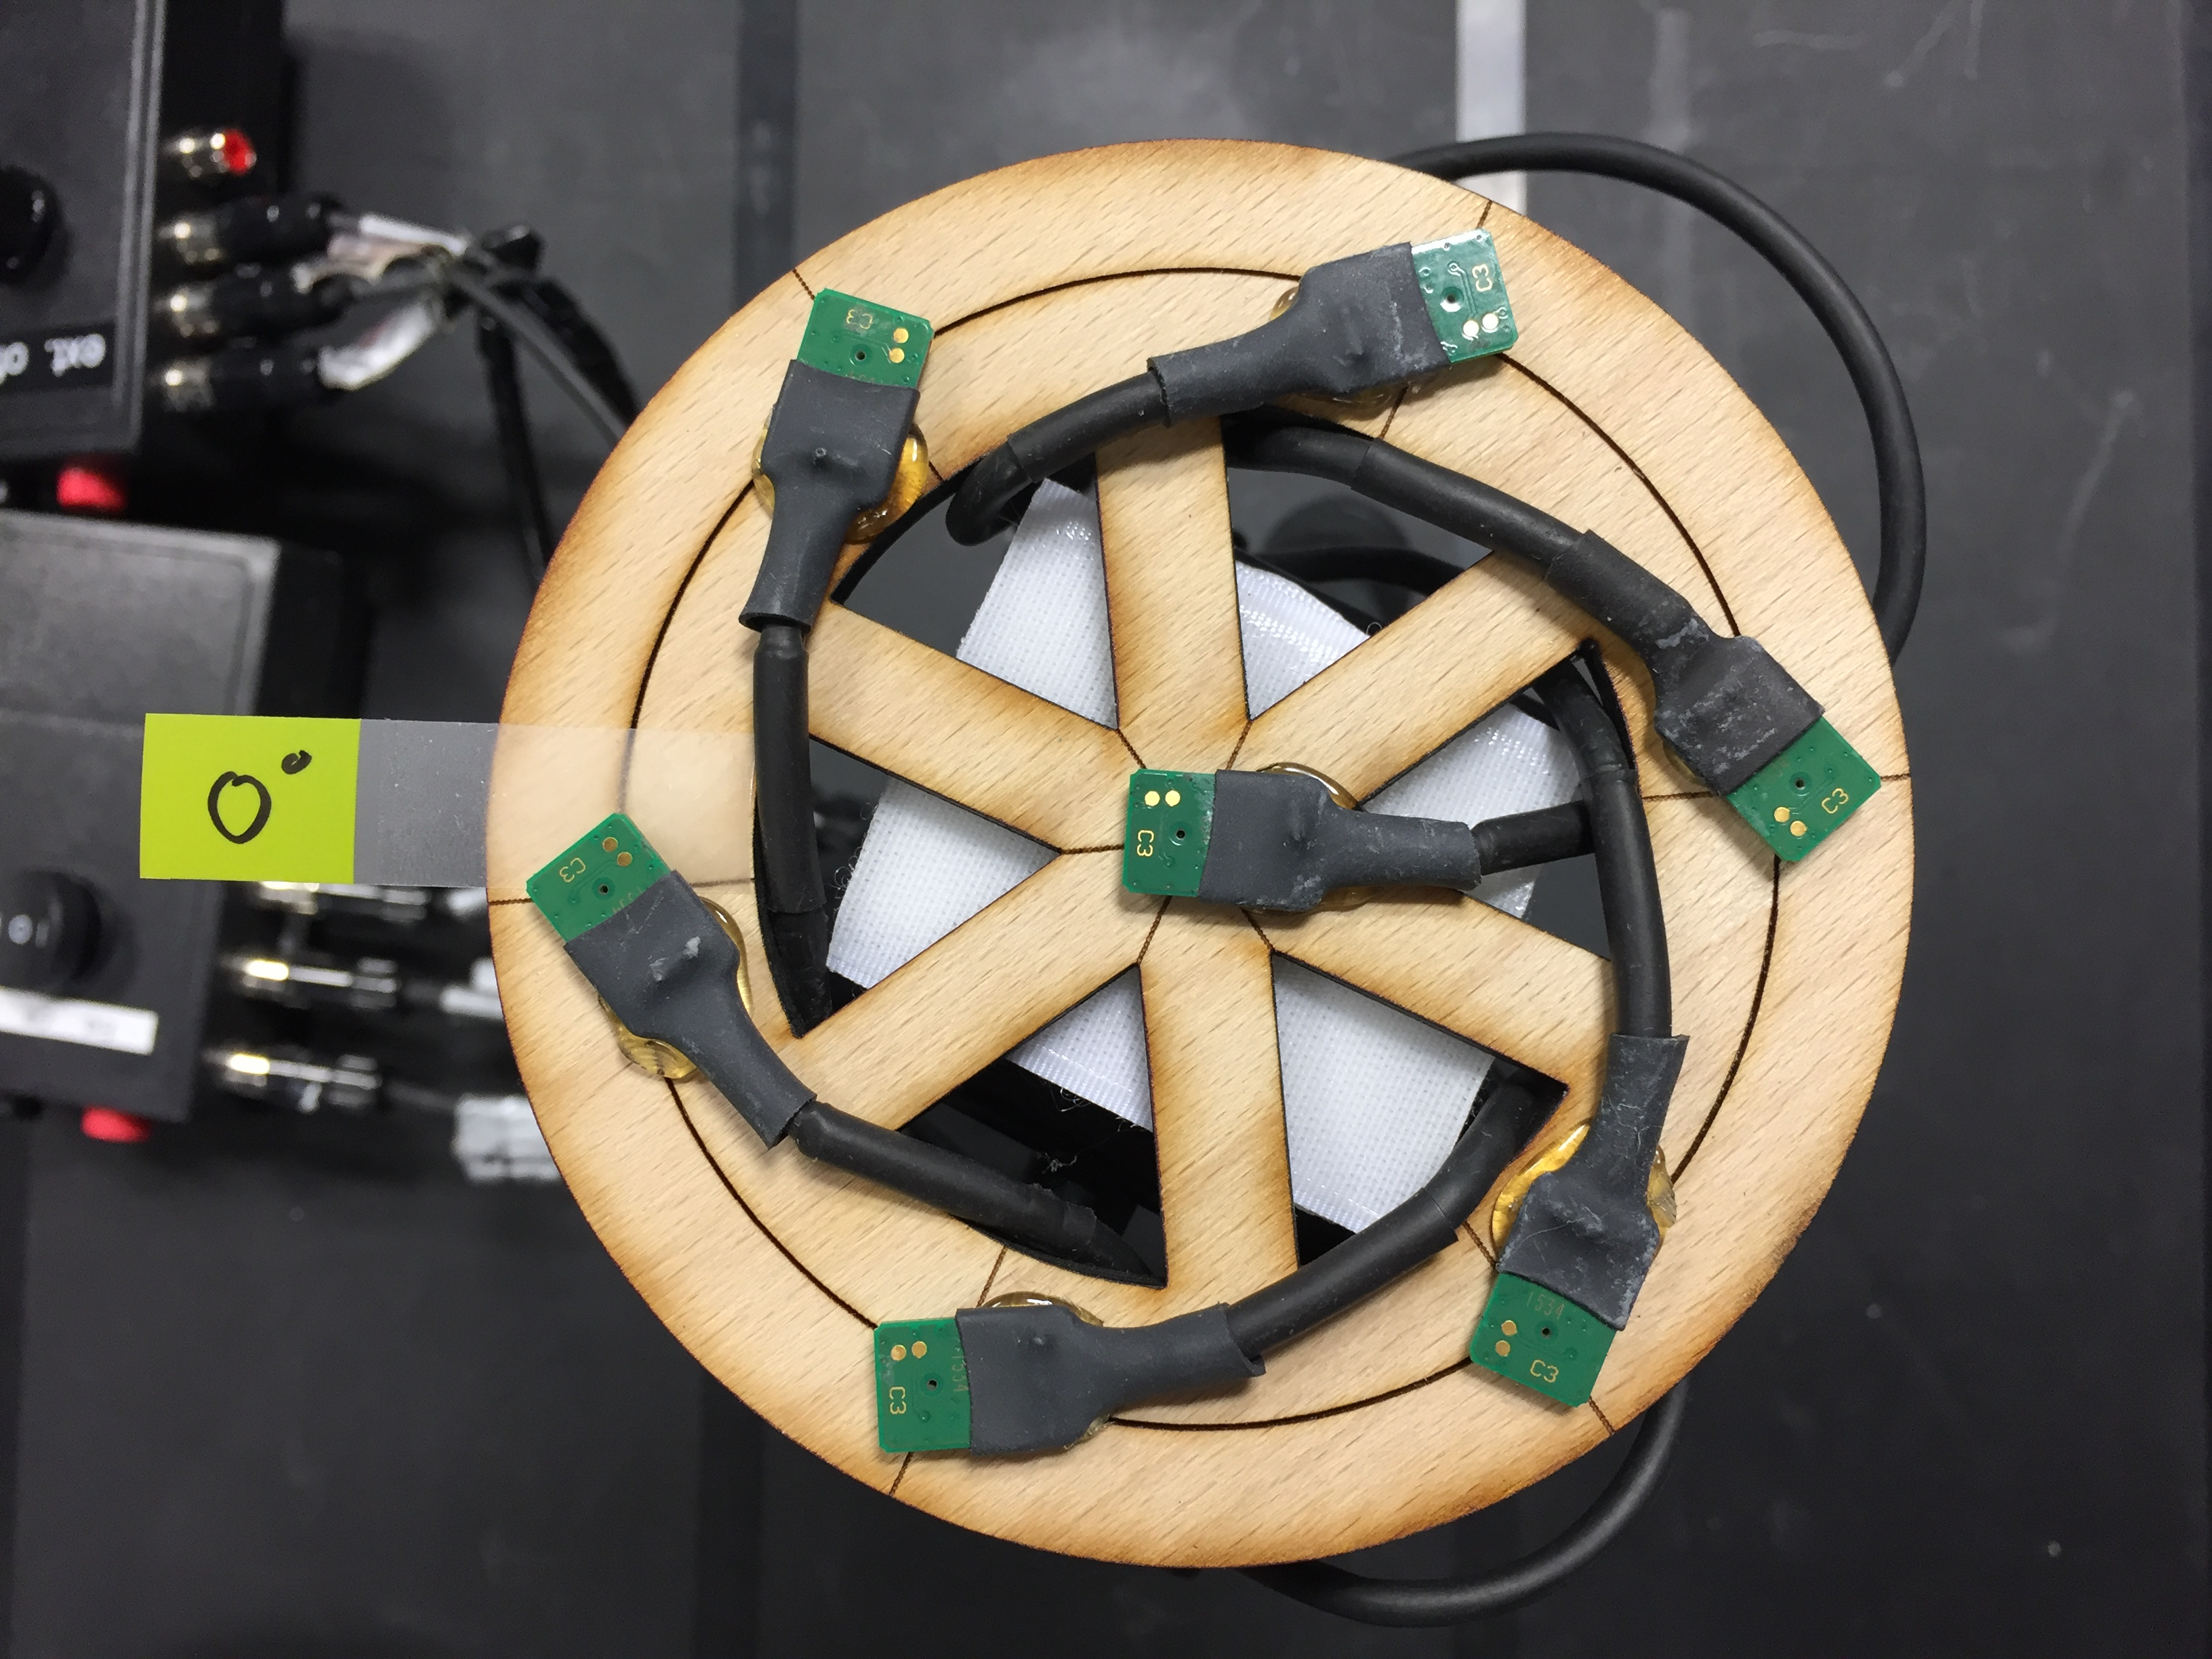
\includegraphics[width=0.8\textwidth]{figures/mic_array_foto.jpg}
	\caption{Foto of the used 7 microphone Uniform circular array with center microphone}
	\label{fig:mic_array}
\end{figure}

\begin{figure}[!ht]
	\centering
	\includegraphics[width=0.8\textwidth]{figures/label_tool.PNG}
	\caption{Labeling Tool}
	\label{fig:label_tool}
\end{figure}


\begin{figure}[!ht]
	\centering
	\begin{minipage}[!ht]{.49\textwidth}
		  \def\svgwidth{1\linewidth}
		  \small\input{figures/scenario_1.pdf_tex}
		\caption{Ground truth over time for scenario 1}
		\label{fig:scenario1}
	\end{minipage}%
	\hfill
	\begin{minipage}[!ht]{.49\textwidth}
		\centering
		\def\svgwidth{1\linewidth}
		\input{figures/scenario_2.pdf_tex}
		\caption{Ground truth over time for scenario 2}
		\label{fig:scenario2}
	\end{minipage}
\end{figure}

\begin{figure}[!ht]
	\centering
	\begin{minipage}[!ht]{.49\textwidth}
		  \def\svgwidth{1\linewidth}
		  \small\input{figures/scenario_3.pdf_tex}
		\caption{Ground truth over time for scenario 3}
		\label{fig:scenario3}
	\end{minipage}%
	\hfill
	\begin{minipage}[!ht]{.49\textwidth}
		\centering
		\def\svgwidth{1\linewidth}
		\input{figures/scenario_4.pdf_tex}

		\caption{Ground truth over time for scenario 4}
		\label{fig:scenario4}
	\end{minipage}
\end{figure}

\begin{figure}[!ht]
	\centering
	\begin{minipage}[!ht]{.49\textwidth}
		  \def\svgwidth{1\linewidth}
		  \small\input{figures/scenario_5.pdf_tex}
		\caption{Ground truth over time for scenario 5}
		\label{fig:scenario5}
	\end{minipage}%
	\hfill
	\begin{minipage}[!ht]{.49\textwidth}
		\centering
		\def\svgwidth{1\linewidth}
		\input{figures/scenario_6.pdf_tex}

		\caption{Ground truth over time for scenario 6}
		\label{fig:scenario6}
	\end{minipage}
\end{figure}

\begin{figure}[!ht]
		\centering
		\def\svgwidth{0.5\linewidth}
		\small\input{figures/scenario_7.pdf_tex}
		\caption{Ground truth over time for scenario 7}
		\label{fig:scenario7}
\end{figure}

\begin{table}[!ht]
\centering
\begin{tabular}{lll}
\toprule
\# 			& Development Set                                              \\ \midrule

D1         & One source moving around the array while speaking                                                                                                      \\
D2         & One source speaks successively from three positions                                                                                                \\
D3         & Two sources from fixed positions speaking successively                                                                                              \\
D4         & \begin{tabular}[c]{@{}l@{}}One fixed permanent music source, one moving source permanently speaking\\   with crossover\end{tabular}             \\
D5         & \begin{tabular}[c]{@{}l@{}}Two sources at $\ang{45}$  azimuth plane\\ alternately speaking first then at the same time\end{tabular}              \\
D6         & One source saying a wake-up-word moves and then asks a question                                                                                       \\
D7         & One source saying a wake-up-word and then asks a question while music is playing                                                                                              \\ \bottomrule
           &                                                                                                                                                    \\
           \toprule
\#         & Evaluation Set                                                                                                                                     \\ \midrule
E1         & Two fixed sources at $\ang{90}$ azimuth plane both simultaneously speaking                                                                                    \\
E2         & One fixed source, one moving source speaking simultaneously                                                                                           \\
E3         & \begin{tabular}[c]{@{}l@{}}One fixed source continuously speaking, one moving source speaking wake-up-\\   words from different directions\end{tabular} \\
E4         & Two sources moving and speaking simultaneously, no crossovers                                                                                       \\
E5         & Two sources moving and speaking simultaneously with crossovers                                                                                      \\
E6         & \begin{tabular}[c]{@{}l@{}}Three static sources continuously speaking with minimum $\ang{80}$ azimuth plane\\   distance\end{tabular}                       \\
E7         & \begin{tabular}[c]{@{}l@{}}Three static sources continuously speaking with minimum $\ang{40}$ azimuth plane\\   distance\end{tabular}     					\\
\bottomrule
\end{tabular}
\caption{List of descriptions of all scenarios used for development and evaluation set}
\label{tab:list_scenario}
\end{table}


\begin{table}[!ht]
\centering
\begin{tabular}{l|ll|ll} \toprule
                       & \multicolumn{2}{l}{Broadband SRP} & \multicolumn{2}{l}{Sub-band SRP} \\ \midrule
Parameter              & Delay and Sum       & Capon       & Delay and Sum       & Capon      \\ \midrule
Circular buffer length $N$ & 16                  & 16          & 257                 & 257        \\
Hypothesis threshold $\Gamma_\text{class}^\text{add}$  & 7                   & 8           & 50                  & 20         \\
PDF Floor class $p_\text{floor}$           & 0.0001              & 0.0001      & 0.01                & 0.001      \\
MAP-Adaption par.  $\beta$               & 40                  & 50          & 50                  & 10         \\
Min. mixing coef. $\Gamma^\text{min}_\text{mix}$             & 0.01                & 0.001       & 0.01                & 0.01       \\
Variance $\sigma^2_\text{const}$        & $13^2$                  & $14^2$          & $10^2$                  & $10^2$         \\
Initial TTL value $b_\text{TTL}^\text{add}$      & 30                  & 30          & 50                  & 50         \\
TTL Threshold  $\Gamma^\text{TTL}_\text{thres}$        & 0.01                & 0.01        & 0.01                & 0.01       \\
TTL increase  $b_\text{TTL}^\text{inc}$              & 30                  & 30          & 8                   & 8          \\
TTL maximum  $\Gamma_\text{TTL}^\text{max}$              & 20                  & 20          & 15                  & 15         \\
Overlap Distance $\Gamma_\text{overlap}$      & 40                  & 40          & 40                  & 40         \\
Aliasing Distance  $\Gamma_\text{al}$    & -                   & -           & 15                  & 15        \\
\bottomrule
\end{tabular}
\caption{Parameters for the different developed multi-source classification algorithm}
\label{tab:para_alg}
\end{table}

\begin{table}[!ht]
\centering

\begin{tabular}{l|l}
\toprule
Parameter Name            & Value \\\midrule
Buffer Length   $N$          & 257   \\
Number of initial sources $K_\text{init}$ & 5     \\
Initial TTL $b_\text{TTL}^\text{init}$              & 2     \\
TTL increase $b_\text{TTL}^\text{inc}$             & 12    \\
TTL maximum  $\Gamma_\text{TTL}^\text{max}$              & 20\\
Threshold Affiliations $\Gamma_\text{affil}$   & 70    \\
Floor class   $p_\text{floor}$            & 0.001 \\
Overlap distance  $\Gamma_\text{overlap}$        & 40    \\
\bottomrule
\end{tabular}
\caption{Parameters for Madhu's multi-source classification algorithm}
\label{tab:para_madhu}
\end{table}


\begin{figure}[!ht]
		\centering
		\def\svgwidth{1\linewidth}
		\small\input{figures/results_idc_example1_comp.pdf_tex}
		\caption{Scenario E7, processed with the developed sub-band algorithm with a Capon beamformer}
		\label{fig:results_idc_ex1_comp}
\end{figure}

\begin{figure}[!ht]
	\subfloat[Broadband processing\label{fig:results_comp_ex2}]{%
		  \def\svgwidth{.49\linewidth}
		  \small\input{figures/results_comp_example2.pdf_tex}
	}
	\hfill
	\subfloat[Sub-band processing\label{fig:results_comp_ex3}]{%
		  \def\svgwidth{.49\linewidth}
		  \small\input{figures/results_comp_example3.pdf_tex}
	}
	\caption{Active system track values over time are shown. Sub-band processing has more active system track values than the broadband processing.}
	\label{fig:results_comp_bb_vs_sb}
\end{figure}

\begin{table}[!ht]
\centering
\begin{tabular}{l|ll|ll|l}
\toprule
      & BB D\&S & BB CAP & SB D\&S & SD CAP & MADHU \\ \midrule
E1    & 0       & 0      & 0       & 0      & 0     \\
E2    & 0       & 0      & 0       & 0      & 0     \\
E3    & 0       & 0      & 0       & 0      & 2     \\
E4    & 0       & 0      & 0       & 0      & 0     \\
E5    & 8       & 6      & 6       & 6      & 6     \\
E6    & 0       & 0      & 0       & 0      & 0     \\
E7    & 8       & 10     & 0       & 0      & 0     \\ \midrule
Total & 16      & 16     & 6       & 6      & 8    \\
\bottomrule
\end{tabular}
\caption{ID changes for all scenarios and algorithms}
\label{tab:idc}
\end{table}

\begin{table}[!ht]
\centering
\begin{tabular}{l|ll|ll|l}
\toprule
      & BB D\&S & BB CAP & SB D\&S & SD CAP & MADHU \\\midrule
E1    & $\ang{3.46 }$   & $\ang{2.86 }$  & $\ang{3.18 }$   & $\ang{3.35 }$  & $\ang{3.35 }$ \\
E2    & $\ang{4.66 }$   & $\ang{4.09 }$  & $\ang{3.64 }$   & $\ang{3.71 }$  & $\ang{5.08 }$ \\
E3    & $\ang{2.78 }$   & $\ang{3.64 }$  & $\ang{1.26 }$   & $\ang{2.05 }$  & $\ang{4.87 }$ \\
E4    & $\ang{4.84 }$   & $\ang{5.09 }$  & $\ang{4.08 }$   & $\ang{3.26 }$  & $\ang{2.89 }$ \\
E5    & $\ang{13.15}$   & $\ang{14.37}$  & $\ang{8.73 }$   & $\ang{9.68 }$  & $\ang{9.42 }$ \\
E6    & $\ang{2.17 }$   & $\ang{2.17 }$  & $\ang{2.45 }$   & $\ang{2.85 }$  & $\ang{3.74 }$ \\
E7    & $\ang{9.69 }$   & $\ang{8.32 }$  & $\ang{1.87 }$   & $\ang{1.99 }$  & $\ang{8.43 }$ \\ \midrule
Total & $\ang{7.62 }$   & $\ang{7.95 }$  & $\ang{4.32 }$   & $\ang{4.92 }$  & $\ang{6.3  }$\\ \bottomrule
\end{tabular}
\caption{Root mean square error values for all scenarios and algorithms}
\label{tab:rmse}
\end{table}

\begin{table}[!ht]
\centering

\begin{tabular}{l|ll|ll|l}
\toprule
      & BB D\&S & BB CAP & SB D\&S & SD CAP & MADHU \\ \midrule
E1    & 1.77    & 2.02   & 0.09    & 0.58   & 0.05  \\
E2    & 0.27    & 0.29   & 0.08    & 0.08   & 0.08  \\
E3    & 0.28    & 0.22   & 0.15    & 0.16   & 0.15  \\
E4    & 0.16    & 0.14   & 0.02    & 0.03   & 0     \\
E5    & 0       & 0      & 0.13    & 0      & 0     \\
E6    & 1.42    & 1.38   & 0.19    & 0.04   & 0.04  \\
E7    & 0.14    & 0.19   & 0       & 0      & 0     \\ \midrule
Total & 0.56    & 0.59   & 0.08    & 0.1    & 0.03  \\ \bottomrule
\end{tabular}
\caption{Initial detection lag in seconds for all scenarios and algorithms}
\label{tab:lag}
\end{table}


\begin{table}[!ht]
\centering
\begin{tabular}{l|ll|ll|l}
\toprule
      & BB D\&S & BB CAP & SB D\&S & SD CAP & MADHU \\\midrule
E1    & 0     & 0      & 0     & 0      & 0     \\
E2    & 0     & 0      & 0     & 0      & 0     \\
E3    & 0     & 0      & 0     & 0      & 0     \\
E4    & 0     & 0      & 0     & 0      & 0     \\
E5    & 1     & 1      & 2     & 2      & 1     \\
E6    & 0     & 0      & 0     & 0      & 0     \\
E7    & 0     & 0      & 0     & 0      & 0     \\ \midrule
Total & 1     & 1      & 2     & 2      & 1    \\
\bottomrule
\end{tabular}
\caption{Interrupt values for all scenarios and algorithms}
\label{tab:interrupts}
\end{table}

\begin{table}[!ht]
\centering
\begin{tabular}{l|ll|ll|l}
\toprule
      & BB D\&S & BB CAP & SB D\&S & SD CAP & MADHU \\ \midrule
E1    & 0       & 0      & 0       & 0      & 0.03  \\
E2    & 0       & 0      & 0       & 0      & 0.43  \\
E3    & 7.1     & 1.66   & 7.06    & 5.9    & 9.79  \\
E4    & 0       & 0      & 0       & 0      & 0     \\
E5    & 0       & 0      & 0       & 1.12   & 0.03  \\
E6    & 0       & 0      & 0.67    & 0.43   & 1.7   \\
E7    & 0       & 0      & 0.5     & 0      & 0.45  \\ \midrule
Total & 7.1     & 1.66   & 8.22    & 7.46   & 12.43   \\
\bottomrule
\end{tabular}
\caption{False positive durations in seconds for all scenarios and algorithms}
\label{tab:fp}
\end{table}

\end{appendix}

